\section{Stage I: Source-Level Optimisation}
\label{sec:stage1}

\subsection{First Numbers}
The first OxCaml port (\code{-O3}, bounds checks on, one accumulator per row;
\code{oxcaml_safe_plain}) is \textbf{$4.19\times$ slower} than
scalar C++ and $4.52\times$ slower than vectorised C++.
Table~\ref{tab:uniform} shows the five ports at the end of the source-level
work, including the hand strength reduction of Section~\ref{sec:sr}.

\begin{table}[h]
  \centering
  \small
  \begin{tabular}{@{}llrrl@{}}
    \toprule
    port & build & tokens/s & vs Python & perplexity \\
    \midrule
    C++    & g++ 14.2 \code{-O3}, unrolled & 772,261 & $119\times$ & 10.789614873329409 \\
    Rust   & rustc 1.98.1 \code{--release}, unrolled & 703,295 & $109\times$ & 10.789614873329409 \\
    OxCaml & 5.4.0-ox7 \code{-O3 -unsafe}, unrolled, hand s.r. & 473,779 & $73\times$ & 10.789614873329409 \\
    OCaml  & 5.3.0 \code{-unsafe}, unrolled, hand s.r. & 448,265 & $69\times$ & 10.789614873329409 \\
    Python & CPython 3.13.5 & 6,479 & $1\times$ & 10.789614873329409 \\
    \bottomrule
  \end{tabular}
  \caption{The five ports' best builds without compiler changes in run W
  (median of 21 interleaved rounds; s.r., strength reduction), all with
  identical output.}
  \label{tab:uniform}
\end{table}

\subsection{Rust: Three Small Changes}
Three changes, each worth a few percent at most and part of every Rust build,
brought Rust level with C++: hoisting the per-layer KV-cache slices out of the
attention loops; iterating \code{linear} with \code{chunks_exact(cols)}, so
the bounds are proved once per row; and precomputing the attention scale (no
measurable effect: LLVM already turns \code{pow(x, 0.5)} into a square root).

\subsection{Fairness Corrections and Bounds Checks}
\label{tab:bounds}
C++ is built with \code{-O3} to match Cargo's opt-level 3 (worth
$+15.3\%$ (21/21) over \code{-O2} on the plain kernel). OCaml's
\code{-unsafe} removes bounds checks, as C++ does by default; Rust keeps its
checks, and LLVM removes them by proof. The price of bounds checks is not
fixed. For stock OCaml on the plain kernel \code{-unsafe} gains only
$+10.0\%$ (20/21), consistent with the checks executing
in the shadow of the single serial chain of additions; on the unrolled kernel
it gains $+29.2\%$ (21/21). For OxCaml the checks are
expensive on both kernels: $+61.6\%$ (21/21) and
$+25.4\%$ (21/21).

\subsection{The Largest Single Change: Unrolling the Rows}
\label{sec:unroll}
Unrolling \code{linear} to compute four rows at once
(Listing~\ref{lst:unrolled}; Section~\ref{sec:bg-ilp}) gave OxCaml
$+56.4\%$ (21/21) and stock OCaml
$+210.6\%$ (21/21), while the same unroll gave C++
$+20.4\%$ (21/21) and Rust only $+5.8\%$ (18/21)
(Figure~\ref{fig:unroll}). The unroll gives four independent accumulators
instead of one, and one load of \code{x.(i)} shared by four rows. Its value
depends on how well each compiler's plain loop already ran: plain Rust is
within $1.07\times$ of scalar C++, plain stock OCaml
$5.48\times$ behind it. Section~\ref{sec:simd-why} tests whether
four chains are enough.

\begin{lstlisting}[language=OCamlX,caption={The shipped OCaml kernel: four rows, four independent accumulators, each row summed left to right (C++ and Rust alike).},label=lst:unrolled]
let linear (x : float array) (w : mat) (out : float array) =
  let cols = w.cols and rows = w.rows and d = w.d in
  let o = ref 0 in
  while !o + 4 <= rows do
    let b0 = !o * cols in
    let b1 = b0 + cols and b2 = b0 + (2 * cols) and b3 = b0 + (3 * cols) in
    let a0 = ref 0.0 and a1 = ref 0.0 and a2 = ref 0.0 and a3 = ref 0.0 in
    for i = 0 to cols - 1 do
      let xi = x.(i) in
      a0 := !a0 +. (d.(b0 + i) *. xi);
      a1 := !a1 +. (d.(b1 + i) *. xi);
      a2 := !a2 +. (d.(b2 + i) *. xi);
      a3 := !a3 +. (d.(b3 + i) *. xi)
    done;
    out.(!o) <- !a0; out.(!o + 1) <- !a1;
    out.(!o + 2) <- !a2; out.(!o + 3) <- !a3;
    o := !o + 4
  done
  (* remainder rows: one accumulator each *)
\end{lstlisting}

\begin{figure}[h]
  \centering
  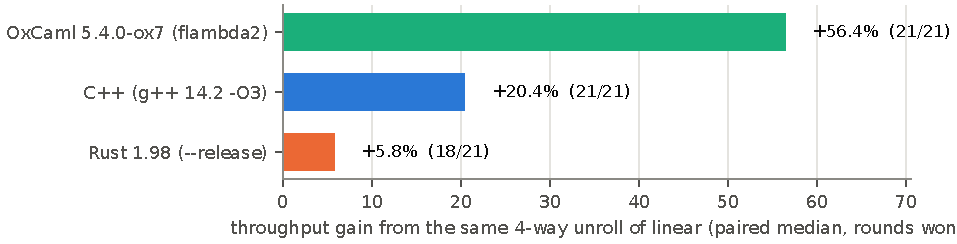
\includegraphics[width=0.78\textwidth]{fig_unroll}
  \caption{The same source change on three compilers (run W, paired median and
  rounds won).}
  \label{fig:unroll}
\end{figure}

\subsection{Two OCaml Compilers}
On the plain kernel flambda2 is $+41.2\%$ (21/21) faster
than the closure middle end ($+108.5\%$ (21/21) with
\code{-unsafe}); on the unrolled kernel it shrinks to
$+4.2\%$ (15/21). On the plain kernel the closure
compiler does not inline the inner loop's local function: it allocates a
closure per row and keeps the accumulator boxed, so each multiply--add costs
21 instructions and 16 bytes of allocation. flambda2 turns it into a loop with
the accumulator in a register (12 instructions, no allocation). The unrolled
kernel is already a loop, and there the two compilers are close.

\subsection{Where Stage I Ended}
OxCaml became $2.54\times$ faster than its first
version, and the gap to scalar C++ fell from $4.19\times$ to
$1.65\times$ ($1.78\times$ to vectorised C++).
Everything after this leaves the OCaml source alone.
